\documentclass[11pt, titlepage]{article}
\usepackage{epsfig,latexsym}
\usepackage{amsmath}
\usepackage{graphicx}
\usepackage{placeins}
\usepackage{fancyhdr}
\usepackage{listings}


\setlength{\textwidth}{7.25in}
\setlength{\textheight}{9.5in}
\setlength{\topmargin}{-0.75in}
\setlength{\oddsidemargin}{-0.5in}
\setlength{\evensidemargin}{-0.5in}
\setlength{\headheight}{26pt}

\lstset{
    basicstyle = \footnotesize,
	breakatwhitespace = false,
	breaklines = true,
	language = C,
	frame=single
	%tabsize=2
}

\pagestyle{fancy}
\fancyhead[R]{EEC 172 Lab3 \\
    			Richard Szeto \& Sean Ho}

\title{EEC 172 Lab3}

\author{Richard Szeto \& Sean Ho}

\date{February 22, 2013}

\begin{document}

    \maketitle
    
    \section{Objectives}
        \subsection{Part A}
            The objectives for Part A is to modify the uart echo code to be able to echo back the data that is inputted into X-CTU to the remote XBee. The input and echo data will be displayed on the X-CTU terminal.
        
        \subsection{Part B}
            The objectives for Part B is to successfully send data from the XBee connected to the LM3S8962 to the XBee connected to the LM3S2110. The input will be from the X-CTU terminal. The status LED from the LM3S2110 will turn on when it receives a '1', and will turn off when it receives a '0'.
        
        \subsection{Part C}
            The objectives for Part C is to send text messages back and forth between the LM3S8962 and the LM3S2110. The IR remotes will be used as the typing medium, and the OLED display of the LM3S8962 will display the messages of the LM3S8962 and the LM3S2110 on a split screen. The LM3S8962 will output the Morse code corresponding to the message it receives.
    
    \section{Procedures}
        \subsection{Part A}
            We modified the uart echo code to fit the specifications of the XBee. We used the X-CTU to test the modified uart echo code. Once X-CTU successfully connected to the XBee, we set both XBees to use our designated PAN and channel numbers. That way the two XBees can communicate with each other without interfering with XBees used by other groups. To verify that the two XBees can communicate with each other, we placed a wire going from Data Out to Data In in the remote XBee. This causes the remote XBee to send out the same data as it receives. If the XBee communication works correctly, the XBee connected to X-CTU should also receive the same data as it sent out and the X-CTU terminal should display and echo of the data that was sent.
        
        \subsection{Part B}
            Now that we know both XBees can communicate with each other, we can test if the XBee connected to the X-CTU can communicate with the LM3S2110 through the remote XBee. The LM3S2110 is to be programmed such that the status light turns on if the remote XBee receives a '1', and the status light turns off if the remote XBee receives a '0'. This can be done by having the LM3S2110 parse in the data coming from the Data Out of the remote XBee.
        
        \subsection{Part C}
            To send a sequence of characters from one XBee to another delimited by the \texttt{ENTER} key on the IR remote, we needed to set both XBees to API mode and designate each XBee with a different source address. The XBee connected to the LM3S8962 would take the 0x0 address and the XBee connected to the LM3S2110 would take the 0x1 address. Since both XBees are in API mode, we need to send packets conforming to the \texttt{Transmit Request:16-bit address} format and receive packets conforming to the \texttt{Receive Packet:16-bit address} format. To correctly send a packet, the sender must create a packet that conforms to the \texttt{Transmit Request:16-bit address} format and send it to the Data In of the connected XBee. The connected XBee will then automatically create a packet that conforms to the \texttt{Receive Packet:16-bit address} format, and send the packet to the Data Out of that XBee and will also send the same packet out into the air. The receiver XBee will accept the packet from the air and output that packet to the Data Out of that XBee. The connected device will parse through the packet to find the payload. The payload will contain the text message that was sent. The LM3S8962 will display both messages that are sent and received by that device by splitting the OLED display into two halves. The top half will represent the text message that is sent by the LM3S8962 and the bottom half will represent the text message that is received by the LM3S8962 (also the same message that was sent by the LM3S2110). The LM3S2110 will display morse code through the use of the status light for messages that are sent and received by that device.
    
    \section{Implementation}
        \textbf{Note}: Only our Part C code is included in this lab report.
        \subsection{Part A}
            \subsubsection{LM3S8962}
                We modified the uart echo code by adding an extra uart interrupt handler for UART1. The original uart echo code already had a uart interrupt handler for UART0, so we did not have to do much modifying for that port. For each uart port, we set the appropriate baud rate, parity, etc. the reflected the specifications of the XBee. We also enabled the hardcoded ports used by UART0 and UART1. To send data out to the XBee, we had to pass data from the UART0 interrupt handler to UART1. To view the echoed data in X-CTU, we had to pass data from the UART1 interrupt handler to UART0. For the UART1 interrupt handler, we did something similar to what was described above.
            
        \subsection{Part B}
            \subsubsection{LM3S8962}
                The same code that was used in Part A was used for Part B.
            
            \subsubsection{LM3S2110}
                We basically copied the code that was used by the LM3S8962 to the LM3S2110. We changed the hardcoded ports that were used by UART0, and there was no UART1 in the LM3S2110, so we removed the corresponding interrupt handler and any of the functions that referred to it. In the while loop of the UART0 interrupt handler, we added an if statement to check for the '1' and '0' characters. If the current character was a '1', then the status light would turn on. If the current character was a '0', then the status light would turn off.
        
        \subsection{Part C}
            \subsubsection{LM3S8962}
                Since Part C involved the IR remote, we integrated our code from Lab2 into our current code for Part C. We modified our lab2 code to include the \texttt{LAST} button, since our TV code does not support the \texttt{ENTER} button. To reflect API mode, we had to create a character array to store all the pieces of information as seen in the Logic Analyzer picture of the Lab3 prompt. To reduce any problems, we removed the code that sent data to UART0. Instead of using the X-CTU, we used the Logic Analyzer for debugging sent and received packets. To extract data from a packet, we would have to find the "size" and "payload" fields of the packet. The payload field size reflected the "size" field we found in the packet. To output the text messages onto the OLED display, we displayed any sent messages from the LM3S8962 onto the top half of the display, and displayed the payload that was received from the LM3S2110 on the bottom half of the display.
            
            \subsubsection{LM3S2110}
                What was described above for the LM3S8962 will be about the same for the LM3S2110, except we display Morse code on the status light instead of displaying text on a display.
    
    \section{Screenshots of XBee Packets}
        \subsection{LM3S8962 is the Sender}
            \FloatBarrier
            \begin{figure}[htbp]
                \centering
                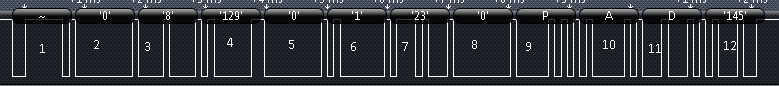
\includegraphics[scale = 0.8]{Screenshots/8962_in.png}
                \caption{LM3S8962 XBee Data In}
            \end{figure}
            \FloatBarrier
            
            \textbf{Legend}
            \begin{itemize}
                \item (1) Start Delimiter
                \item (2 - 3) Length of Frame Data
                \item (4 - 11) Frame Data
                    \begin{itemize}
                        \item (4) API Identifier
                        \item (5 - 11) Identifier-specific Data
                            \begin{itemize}
                                \item (5) Frame ID
                                \item (6 - 7) Destination Address
                                \item (8) Options
                                \item (9 - 11) RF Data (Payload)
                            \end{itemize}
                    \end{itemize}
                \item (12) Checksum
            \end{itemize}
            
            \FloatBarrier
            \begin{figure}[htbp]
                \centering
                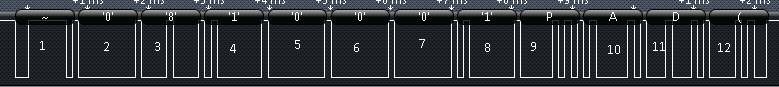
\includegraphics[scale = 0.8]{Screenshots/2110_out.png}
                \caption{LM3S2110 XBee Data Out}
            \end{figure}
            \FloatBarrier
            
            \textbf{Legend}
            \begin{itemize}
                \item (1) Start Delimiter
                \item (2 - 3) Length of Frame Data
                \item (4 - 11) Frame Data
                    \begin{itemize}
                        \item (4) API Identifier
                        \item (5 - 11) Identifier-specific Data
                            \begin{itemize}
                                \item (5 - 6) Source Address
                                \item (7) Received Signal Strength Indicator
                                \item (8) Options
                                \item (9 - 11) RF Data (Payload)
                            \end{itemize}
                    \end{itemize}
                \item (12) Checksum
            \end{itemize}
        
        \subsection{LM3S2110 is the Sender}
            \FloatBarrier
            \begin{figure}[htbp]
                \centering
                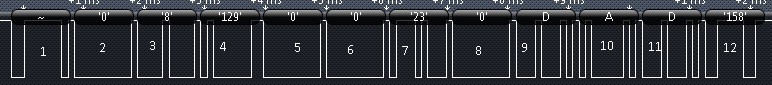
\includegraphics[scale = 0.8]{Screenshots/2110_in.png}
                \caption{LM3S2110 XBee Data In}
            \end{figure}
            \FloatBarrier
            
            \textbf{Legend}
            \begin{itemize}
                \item (1) Start Delimiter
                \item (2 - 3) Length of Frame Data
                \item (4 - 11) Frame Data
                    \begin{itemize}
                        \item (4) API Identifier
                        \item (5 - 11) Identifier-specific Data
                            \begin{itemize}
                                \item (5) Frame ID
                                \item (6 - 7) Destination Address
                                \item (8) Options
                                \item (9 - 11) RF Data (Payload)
                            \end{itemize}
                    \end{itemize}
                \item (12) Checksum
            \end{itemize}
            
            \FloatBarrier
            \begin{figure}[htbp]
                \centering
                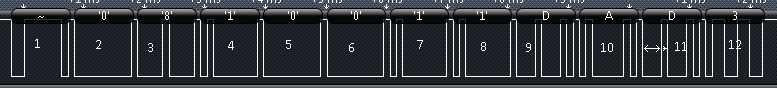
\includegraphics[scale = 0.8]{Screenshots/8962_out.png}
                \caption{LM3S8962 XBee Data Out}
            \end{figure}
            \FloatBarrier
            
            \textbf{Legend}
            \begin{itemize}
                \item (1) Start Delimiter
                \item (2 - 3) Length of Frame Data
                \item (4 - 11) Frame Data
                    \begin{itemize}
                        \item (4) API Identifier
                        \item (5 - 11) Identifier-specific Data
                            \begin{itemize}
                                \item (5 - 6) Source Address
                                \item (7) Received Signal Strength Indicator
                                \item (8) Options
                                \item (9 - 11) RF Data (Payload)
                            \end{itemize}
                    \end{itemize}
                \item (12) Checksum
            \end{itemize}
    
    \section{Difficulties}
        \subsection{Part A}
            Initially we were unsure of the ports that were used by UART0 and UART1 on the LM3S8962. We did not know at the time that Uart ports are hard coded, so we arbitrarily chose 4 unused ports to map Uart to. We later found out that UART0 was mapped to the mini-USB and UART1 was mapped to ports A01 and A02 on the LM3S8962.
            
        \subsection{Part B}
            After finding the correct Uart ports for the LM3S8962, we searched for the hardcoded Uart ports on the LM3S2110. Initially we found that the Uart ports are mapped on the same pins as the Ulink. We found it inconvenient to constantly add and remove the Ulink from the board whenever we wanted to program or test the board. Later we found out that the same Uart ports found in the pins used by the Ulink can also be found in other parts of the chip. Finding those pins were vital to minimize the time it took to finish this portion of the lab.
        
        \subsection{Part C}
            We initially had no clue how the \texttt{Transmit Request:16-bit address} and the \texttt{Receive Packet:16-bit address} formats worked. The use of trial and error before we understood the required formats wasted a large amount of valuable time. After realizing that the Logic Analyzer picture on the Lab3 prompt represented the correct format, we finally understood what needed to be done. We later found some inconsistent assumptions. The \texttt{UARTCharGet} function used in the LM3S8962 returned the bytes in the payload without first going through the bytes before the payload. However, the \texttt{UARTCharGet} function used in the LM3S2110 returned the bytes expected from the format. The confusion led to a heated discussion and more wasted time. In the end, we accepted this inconsistency and integrated it into our final code.
            
    \section{Miscellaneous}
        The LM3S8962 OLED display will display an error message corresponding to the device that produced the error. The LM3S8962 is directed connected to the OLED display, so the error message will be displayed in real time if there is an invalid button press. The LM3S8962 does not know about any error button presses on the LM3S2110 until a message is sent to the LM3S8962, so an error message can only be displayed when a message is sent from the LM3S2110 to the LM3S8962.
    
    \appendix
    \section{Code for Lab3}
        \subsection{LM3S8962}
            \lstinputlisting{Code/Lab3_8962.c}
        \subsection{LM3S2110}
            \lstinputlisting{Code/Lab3_2110.c}

\end{document}

